\documentclass{article}
\usepackage{graphicx}
\usepackage[margin=1.5cm]{geometry}
\usepackage{amsmath}

\begin{document}

\title{Tuesday Reading Assessment: Unit 4, Field Induction and Inductance}
\author{Prof. Jordan C. Hanson}

\maketitle

\section{Memory Bank}

\begin{itemize}
\item $\epsilon = -N \Delta \phi_m /\Delta t$ ... Faraday's Law, with flux $\phi$
\item $\epsilon = -L \Delta I/\Delta t$ ... Faraday's Law, with inductance $L$
\item $\epsilon_2/\epsilon_1 = N_2/N_1$ ... Transformer equation
\item $\epsilon(t) = \epsilon_0 (2 \pi f) \cos(2\pi ft)$ ... Variation of induced voltage as a function of time and frequency.
\end{itemize}

\begin{figure}[hb]
\centering
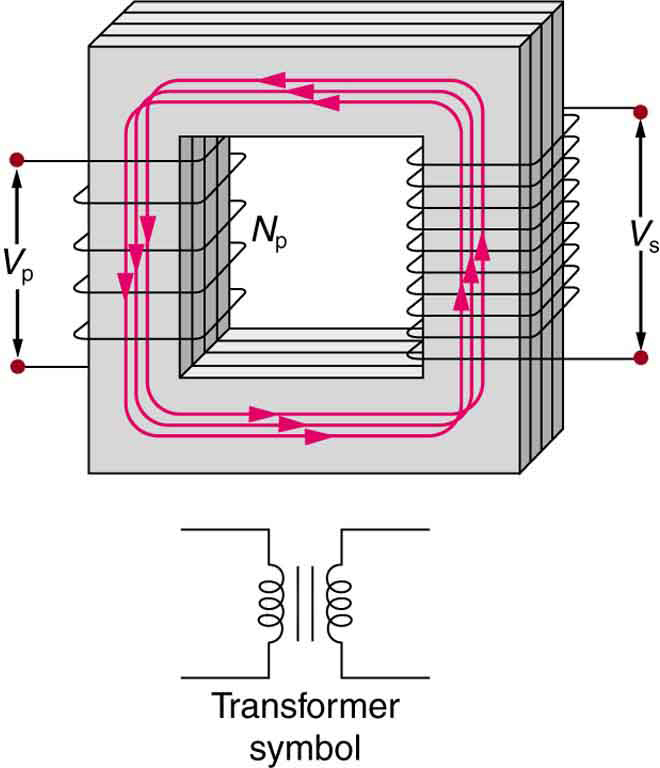
\includegraphics[width=0.2\textwidth]{transformer.jpeg}
\caption{\label{fig:trans} A basic diagram of a transformer with transmit and receive coils.}
\end{figure}

\section{Faraday's Law, Transformers, and Scaling Properties}

\begin{enumerate}
\item Consider Fig. \ref{fig:trans}, which depicts a \textit{transformer.}  There are two solenoids, the \textit{transmit} and \textit{receive} coils.  Using Faraday's law at constant frequency, convince yourself that
\begin{equation}
\frac{\epsilon_{TX}}{\epsilon_{RX}} = \frac{N_{TX}}{N_{RX}}
\end{equation}
\item A battery charger meant for a series connection of ten nickel-cadmium batteries (total emf of 12.5 V DC) needs to have a 15.0 V output to charge the batteries. It uses a step-down transformer with a 200-loop primary and a 120 V input. (a) How many loops should there be in the secondary coil? (b) If the input current is 16.0 A, what is the output current? \\ \vspace{2cm}
\item Suppose Fig. \ref{fig:trans} represents our Faraday's Law lab activity (using an iron core to connect the flux rather than overlapping the coils).  (a) If we observe $\epsilon_{RX}(t) = 5.0\cos(2\pi ft)$ Volts, with $f = 1$ kHz, what will $\epsilon_{RX}(t)$ be at $f = 5$ kHz? (b) What is the period of $\epsilon_{RX}(t)$ when $f = 5$ kHz?
\end{enumerate}

\end{document}
